%==============================================================================
% Figure: Cayley-Dickson Doubling Sequence with Property Loss Cascade
% Source: Ch02 (Cayley-Dickson Algebras)
% Framework: M (Mathematical) | Type: Tree diagram
% Date: 2025-10-21
%==============================================================================

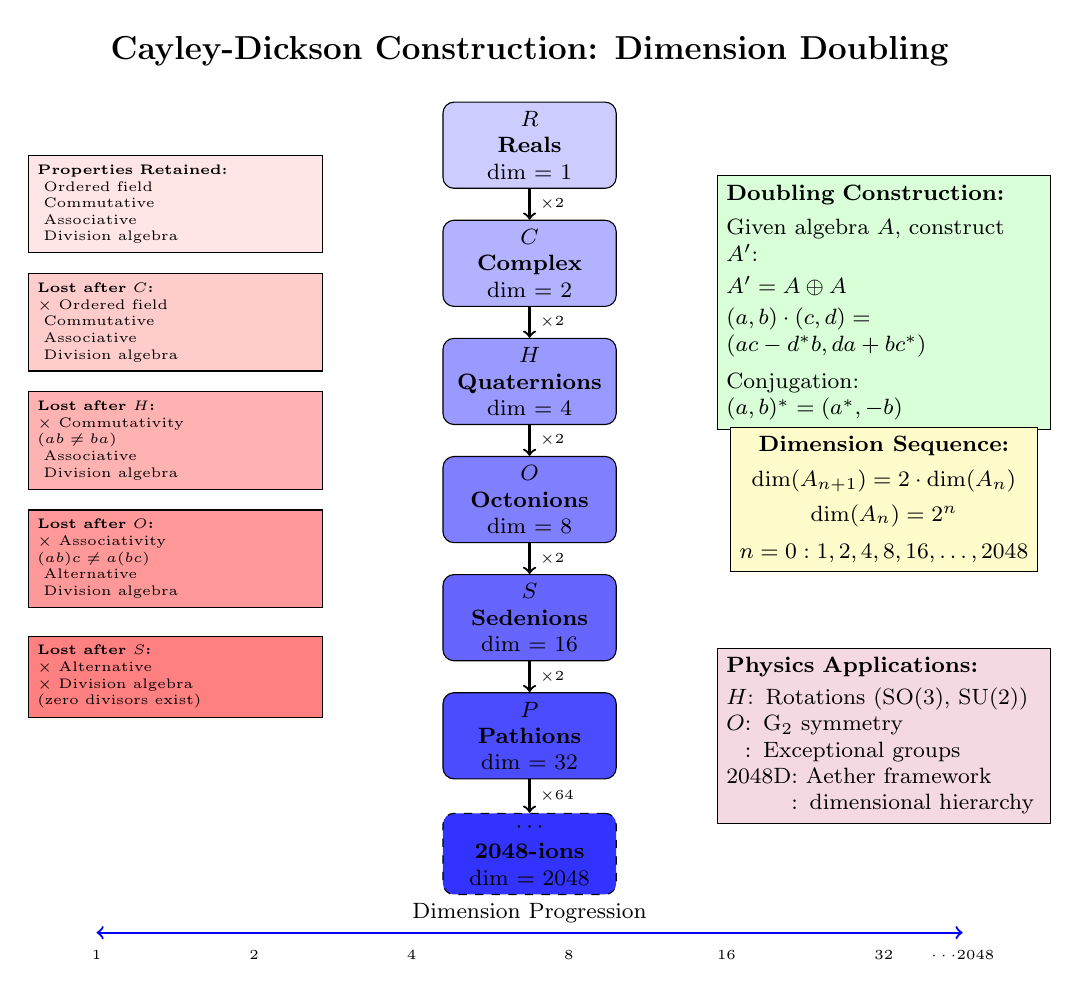
\begin{tikzpicture}[scale=1.0,
  algebra/.style={draw, rectangle, rounded corners, minimum width=2.2cm, minimum height=1cm, font=\footnotesize, align=center},
  property/.style={font=\tiny, text=red},
  arrow/.style={->, thick}]

  % Title
  \node[anchor=north, font=\large\bfseries] at (6,9.5) {Cayley-Dickson Construction: Dimension Doubling};

  % Level 0: Reals
  \node[algebra, fill=blue!20] (R) at (6,8) {
    $\mathbb{R}$ \\
    \textbf{Reals} \\
    dim = 1
  };

  % Level 1: Complex
  \node[algebra, fill=blue!30] (C) at (6,6.5) {
    $\mathbb{C}$ \\
    \textbf{Complex} \\
    dim = 2
  };

  % Level 2: Quaternions
  \node[algebra, fill=blue!40] (H) at (6,5) {
    $\mathbb{H}$ \\
    \textbf{Quaternions} \\
    dim = 4
  };

  % Level 3: Octonions
  \node[algebra, fill=blue!50] (O) at (6,3.5) {
    $\mathbb{O}$ \\
    \textbf{Octonions} \\
    dim = 8
  };

  % Level 4: Sedenions
  \node[algebra, fill=blue!60] (S) at (6,2) {
    $\mathbb{S}$ \\
    \textbf{Sedenions} \\
    dim = 16
  };

  % Level 5: Pathions
  \node[algebra, fill=blue!70] (P) at (6,0.5) {
    $\mathbb{P}$ \\
    \textbf{Pathions} \\
    dim = 32
  };

  % Level 6: Continuation
  \node[algebra, fill=blue!80, dashed] (dots) at (6,-1) {
    $\cdots$ \\
    \textbf{2048-ions} \\
    dim = 2048
  };

  % Arrows with doubling annotation
  \draw[arrow] (R) -- (C) node[midway, right, font=\tiny] {$\times 2$};
  \draw[arrow] (C) -- (H) node[midway, right, font=\tiny] {$\times 2$};
  \draw[arrow] (H) -- (O) node[midway, right, font=\tiny] {$\times 2$};
  \draw[arrow] (O) -- (S) node[midway, right, font=\tiny] {$\times 2$};
  \draw[arrow] (S) -- (P) node[midway, right, font=\tiny] {$\times 2$};
  \draw[arrow] (P) -- (dots) node[midway, right, font=\tiny] {$\times 64$};

  % Property loss cascade (LEFT SIDE)
  \node[draw, rectangle, fill=red!10, font=\tiny, align=left, text width=3.5cm] at (1.5,7.25) {
    \textbf{Properties Retained:} \\
    $\checkmark$ Ordered field \\
    $\checkmark$ Commutative \\
    $\checkmark$ Associative \\
    $\checkmark$ Division algebra
  };

  \node[draw, rectangle, fill=red!20, font=\tiny, align=left, text width=3.5cm] at (1.5,5.75) {
    \textbf{Lost after $\mathbb{C}$:} \\
    $\times$ Ordered field \\
    $\checkmark$ Commutative \\
    $\checkmark$ Associative \\
    $\checkmark$ Division algebra
  };

  \node[draw, rectangle, fill=red!30, font=\tiny, align=left, text width=3.5cm] at (1.5,4.25) {
    \textbf{Lost after $\mathbb{H}$:} \\
    $\times$ Commutativity \\
    $(ab \neq ba)$ \\
    $\checkmark$ Associative \\
    $\checkmark$ Division algebra
  };

  \node[draw, rectangle, fill=red!40, font=\tiny, align=left, text width=3.5cm] at (1.5,2.75) {
    \textbf{Lost after $\mathbb{O}$:} \\
    $\times$ Associativity \\
    $(ab)c \neq a(bc)$ \\
    $\checkmark$ Alternative \\
    $\checkmark$ Division algebra
  };

  \node[draw, rectangle, fill=red!50, font=\tiny, align=left, text width=3.5cm] at (1.5,1.25) {
    \textbf{Lost after $\mathbb{S}$:} \\
    $\times$ Alternative \\
    $\times$ Division algebra \\
    (zero divisors exist)
  };

  % Construction formula (RIGHT SIDE)
  \node[draw, rectangle, fill=green!15, font=\footnotesize, align=left, text width=4cm] at (10.5,6) {
    \textbf{Doubling Construction:} \\[3pt]
    Given algebra $A$, construct $A'$: \\[2pt]
    $A' = A \oplus A$ \\[2pt]
    $(a,b) \cdot (c,d) = $ \\
    $(ac - d^* b, da + bc^*)$ \\[4pt]
    Conjugation: \\
    $(a,b)^* = (a^*, -b)$
  };

  % Dimension formula
  \node[draw, rectangle, fill=yellow!20, font=\footnotesize, align=center] at (10.5,3.5) {
    \textbf{Dimension Sequence:} \\[3pt]
    $\dim(A_{n+1}) = 2 \cdot \dim(A_n)$ \\[3pt]
    $\dim(A_n) = 2^n$ \\[4pt]
    $n=0: 1, 2, 4, 8, 16, \ldots, 2048$
  };

  % Physics applications box
  \node[draw, rectangle, fill=purple!15, font=\footnotesize, align=left, text width=4cm] at (10.5,0.5) {
    \textbf{Physics Applications:} \\[2pt]
    $\mathbb{H}$: Rotations (SO(3), SU(2)) \\
    $\mathbb{O}$: G$_2$ symmetry \\
    \phantom{$\mathbb{O}$}: Exceptional groups \\
    2048D: Aether framework \\
    \phantom{2048D}: dimensional hierarchy
  };

  % Visual dimension progression
  \draw[thick, blue, <->] (0.5,-2) -- (11.5,-2);
  \node[below, font=\tiny] at (0.5,-2.1) {1};
  \node[below, font=\tiny] at (2.5,-2.1) {2};
  \node[below, font=\tiny] at (4.5,-2.1) {4};
  \node[below, font=\tiny] at (6.5,-2.1) {8};
  \node[below, font=\tiny] at (8.5,-2.1) {16};
  \node[below, font=\tiny] at (10.5,-2.1) {32};
  \node[below, font=\tiny] at (11.5,-2.1) {$\cdots$2048};
  \node[above, font=\footnotesize] at (6,-2) {Dimension Progression};

\end{tikzpicture}

% Usage: %==============================================================================
% Figure: Cayley-Dickson Doubling Sequence with Property Loss Cascade
% Source: Ch02 (Cayley-Dickson Algebras)
% Framework: M (Mathematical) | Type: Tree diagram
% Date: 2025-10-21
%==============================================================================

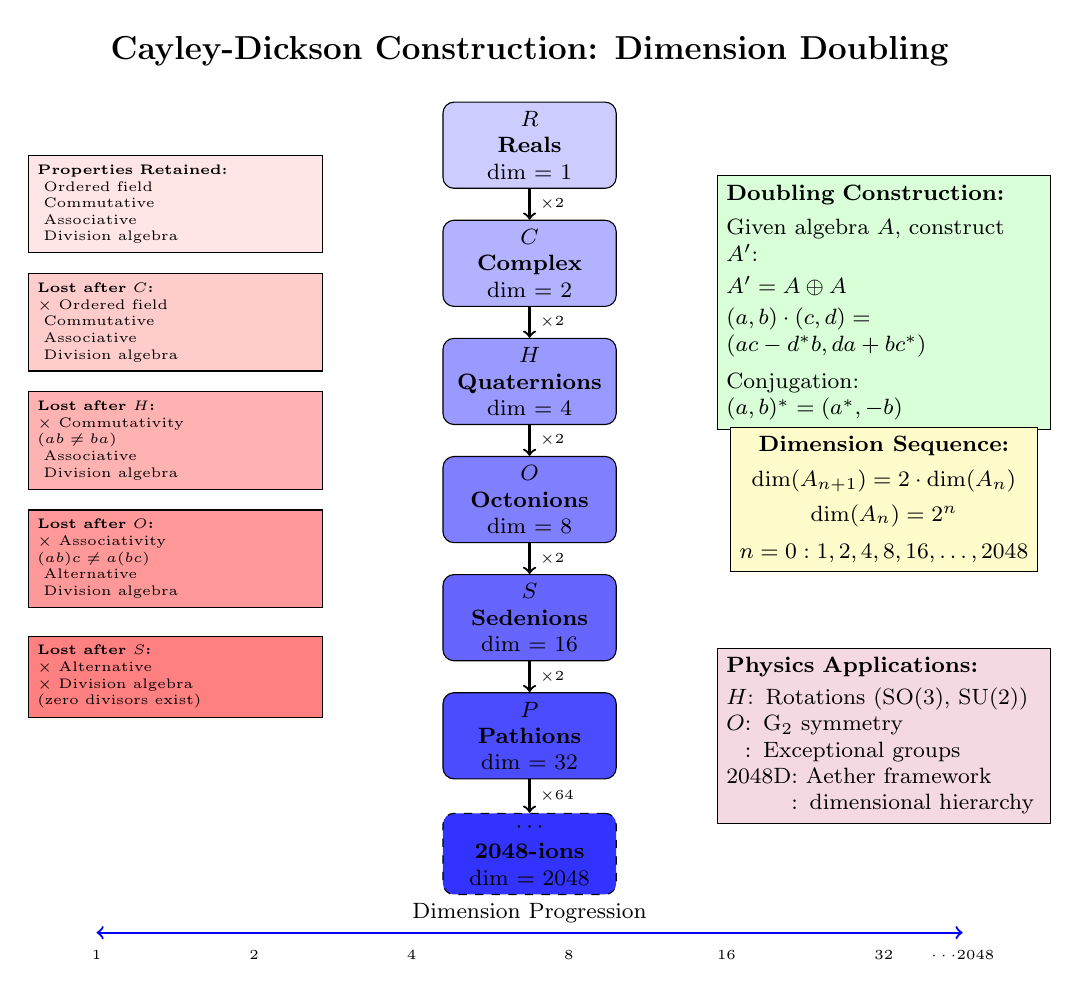
\begin{tikzpicture}[scale=1.0,
  algebra/.style={draw, rectangle, rounded corners, minimum width=2.2cm, minimum height=1cm, font=\footnotesize, align=center},
  property/.style={font=\tiny, text=red},
  arrow/.style={->, thick}]

  % Title
  \node[anchor=north, font=\large\bfseries] at (6,9.5) {Cayley-Dickson Construction: Dimension Doubling};

  % Level 0: Reals
  \node[algebra, fill=blue!20] (R) at (6,8) {
    $\mathbb{R}$ \\
    \textbf{Reals} \\
    dim = 1
  };

  % Level 1: Complex
  \node[algebra, fill=blue!30] (C) at (6,6.5) {
    $\mathbb{C}$ \\
    \textbf{Complex} \\
    dim = 2
  };

  % Level 2: Quaternions
  \node[algebra, fill=blue!40] (H) at (6,5) {
    $\mathbb{H}$ \\
    \textbf{Quaternions} \\
    dim = 4
  };

  % Level 3: Octonions
  \node[algebra, fill=blue!50] (O) at (6,3.5) {
    $\mathbb{O}$ \\
    \textbf{Octonions} \\
    dim = 8
  };

  % Level 4: Sedenions
  \node[algebra, fill=blue!60] (S) at (6,2) {
    $\mathbb{S}$ \\
    \textbf{Sedenions} \\
    dim = 16
  };

  % Level 5: Pathions
  \node[algebra, fill=blue!70] (P) at (6,0.5) {
    $\mathbb{P}$ \\
    \textbf{Pathions} \\
    dim = 32
  };

  % Level 6: Continuation
  \node[algebra, fill=blue!80, dashed] (dots) at (6,-1) {
    $\cdots$ \\
    \textbf{2048-ions} \\
    dim = 2048
  };

  % Arrows with doubling annotation
  \draw[arrow] (R) -- (C) node[midway, right, font=\tiny] {$\times 2$};
  \draw[arrow] (C) -- (H) node[midway, right, font=\tiny] {$\times 2$};
  \draw[arrow] (H) -- (O) node[midway, right, font=\tiny] {$\times 2$};
  \draw[arrow] (O) -- (S) node[midway, right, font=\tiny] {$\times 2$};
  \draw[arrow] (S) -- (P) node[midway, right, font=\tiny] {$\times 2$};
  \draw[arrow] (P) -- (dots) node[midway, right, font=\tiny] {$\times 64$};

  % Property loss cascade (LEFT SIDE)
  \node[draw, rectangle, fill=red!10, font=\tiny, align=left, text width=3.5cm] at (1.5,7.25) {
    \textbf{Properties Retained:} \\
    $\checkmark$ Ordered field \\
    $\checkmark$ Commutative \\
    $\checkmark$ Associative \\
    $\checkmark$ Division algebra
  };

  \node[draw, rectangle, fill=red!20, font=\tiny, align=left, text width=3.5cm] at (1.5,5.75) {
    \textbf{Lost after $\mathbb{C}$:} \\
    $\times$ Ordered field \\
    $\checkmark$ Commutative \\
    $\checkmark$ Associative \\
    $\checkmark$ Division algebra
  };

  \node[draw, rectangle, fill=red!30, font=\tiny, align=left, text width=3.5cm] at (1.5,4.25) {
    \textbf{Lost after $\mathbb{H}$:} \\
    $\times$ Commutativity \\
    $(ab \neq ba)$ \\
    $\checkmark$ Associative \\
    $\checkmark$ Division algebra
  };

  \node[draw, rectangle, fill=red!40, font=\tiny, align=left, text width=3.5cm] at (1.5,2.75) {
    \textbf{Lost after $\mathbb{O}$:} \\
    $\times$ Associativity \\
    $(ab)c \neq a(bc)$ \\
    $\checkmark$ Alternative \\
    $\checkmark$ Division algebra
  };

  \node[draw, rectangle, fill=red!50, font=\tiny, align=left, text width=3.5cm] at (1.5,1.25) {
    \textbf{Lost after $\mathbb{S}$:} \\
    $\times$ Alternative \\
    $\times$ Division algebra \\
    (zero divisors exist)
  };

  % Construction formula (RIGHT SIDE)
  \node[draw, rectangle, fill=green!15, font=\footnotesize, align=left, text width=4cm] at (10.5,6) {
    \textbf{Doubling Construction:} \\[3pt]
    Given algebra $A$, construct $A'$: \\[2pt]
    $A' = A \oplus A$ \\[2pt]
    $(a,b) \cdot (c,d) = $ \\
    $(ac - d^* b, da + bc^*)$ \\[4pt]
    Conjugation: \\
    $(a,b)^* = (a^*, -b)$
  };

  % Dimension formula
  \node[draw, rectangle, fill=yellow!20, font=\footnotesize, align=center] at (10.5,3.5) {
    \textbf{Dimension Sequence:} \\[3pt]
    $\dim(A_{n+1}) = 2 \cdot \dim(A_n)$ \\[3pt]
    $\dim(A_n) = 2^n$ \\[4pt]
    $n=0: 1, 2, 4, 8, 16, \ldots, 2048$
  };

  % Physics applications box
  \node[draw, rectangle, fill=purple!15, font=\footnotesize, align=left, text width=4cm] at (10.5,0.5) {
    \textbf{Physics Applications:} \\[2pt]
    $\mathbb{H}$: Rotations (SO(3), SU(2)) \\
    $\mathbb{O}$: G$_2$ symmetry \\
    \phantom{$\mathbb{O}$}: Exceptional groups \\
    2048D: Aether framework \\
    \phantom{2048D}: dimensional hierarchy
  };

  % Visual dimension progression
  \draw[thick, blue, <->] (0.5,-2) -- (11.5,-2);
  \node[below, font=\tiny] at (0.5,-2.1) {1};
  \node[below, font=\tiny] at (2.5,-2.1) {2};
  \node[below, font=\tiny] at (4.5,-2.1) {4};
  \node[below, font=\tiny] at (6.5,-2.1) {8};
  \node[below, font=\tiny] at (8.5,-2.1) {16};
  \node[below, font=\tiny] at (10.5,-2.1) {32};
  \node[below, font=\tiny] at (11.5,-2.1) {$\cdots$2048};
  \node[above, font=\footnotesize] at (6,-2) {Dimension Progression};

\end{tikzpicture}

% Usage: %==============================================================================
% Figure: Cayley-Dickson Doubling Sequence with Property Loss Cascade
% Source: Ch02 (Cayley-Dickson Algebras)
% Framework: M (Mathematical) | Type: Tree diagram
% Date: 2025-10-21
%==============================================================================

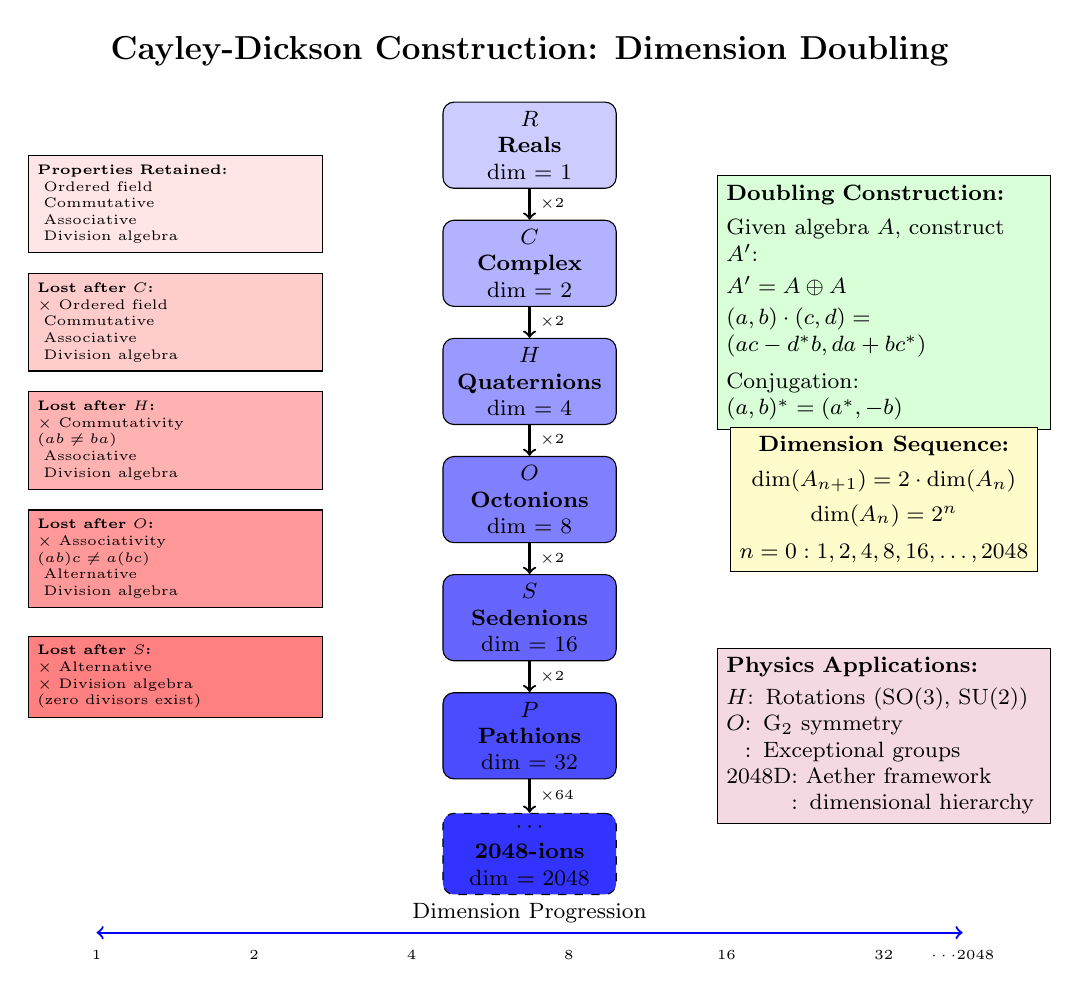
\begin{tikzpicture}[scale=1.0,
  algebra/.style={draw, rectangle, rounded corners, minimum width=2.2cm, minimum height=1cm, font=\footnotesize, align=center},
  property/.style={font=\tiny, text=red},
  arrow/.style={->, thick}]

  % Title
  \node[anchor=north, font=\large\bfseries] at (6,9.5) {Cayley-Dickson Construction: Dimension Doubling};

  % Level 0: Reals
  \node[algebra, fill=blue!20] (R) at (6,8) {
    $\mathbb{R}$ \\
    \textbf{Reals} \\
    dim = 1
  };

  % Level 1: Complex
  \node[algebra, fill=blue!30] (C) at (6,6.5) {
    $\mathbb{C}$ \\
    \textbf{Complex} \\
    dim = 2
  };

  % Level 2: Quaternions
  \node[algebra, fill=blue!40] (H) at (6,5) {
    $\mathbb{H}$ \\
    \textbf{Quaternions} \\
    dim = 4
  };

  % Level 3: Octonions
  \node[algebra, fill=blue!50] (O) at (6,3.5) {
    $\mathbb{O}$ \\
    \textbf{Octonions} \\
    dim = 8
  };

  % Level 4: Sedenions
  \node[algebra, fill=blue!60] (S) at (6,2) {
    $\mathbb{S}$ \\
    \textbf{Sedenions} \\
    dim = 16
  };

  % Level 5: Pathions
  \node[algebra, fill=blue!70] (P) at (6,0.5) {
    $\mathbb{P}$ \\
    \textbf{Pathions} \\
    dim = 32
  };

  % Level 6: Continuation
  \node[algebra, fill=blue!80, dashed] (dots) at (6,-1) {
    $\cdots$ \\
    \textbf{2048-ions} \\
    dim = 2048
  };

  % Arrows with doubling annotation
  \draw[arrow] (R) -- (C) node[midway, right, font=\tiny] {$\times 2$};
  \draw[arrow] (C) -- (H) node[midway, right, font=\tiny] {$\times 2$};
  \draw[arrow] (H) -- (O) node[midway, right, font=\tiny] {$\times 2$};
  \draw[arrow] (O) -- (S) node[midway, right, font=\tiny] {$\times 2$};
  \draw[arrow] (S) -- (P) node[midway, right, font=\tiny] {$\times 2$};
  \draw[arrow] (P) -- (dots) node[midway, right, font=\tiny] {$\times 64$};

  % Property loss cascade (LEFT SIDE)
  \node[draw, rectangle, fill=red!10, font=\tiny, align=left, text width=3.5cm] at (1.5,7.25) {
    \textbf{Properties Retained:} \\
    $\checkmark$ Ordered field \\
    $\checkmark$ Commutative \\
    $\checkmark$ Associative \\
    $\checkmark$ Division algebra
  };

  \node[draw, rectangle, fill=red!20, font=\tiny, align=left, text width=3.5cm] at (1.5,5.75) {
    \textbf{Lost after $\mathbb{C}$:} \\
    $\times$ Ordered field \\
    $\checkmark$ Commutative \\
    $\checkmark$ Associative \\
    $\checkmark$ Division algebra
  };

  \node[draw, rectangle, fill=red!30, font=\tiny, align=left, text width=3.5cm] at (1.5,4.25) {
    \textbf{Lost after $\mathbb{H}$:} \\
    $\times$ Commutativity \\
    $(ab \neq ba)$ \\
    $\checkmark$ Associative \\
    $\checkmark$ Division algebra
  };

  \node[draw, rectangle, fill=red!40, font=\tiny, align=left, text width=3.5cm] at (1.5,2.75) {
    \textbf{Lost after $\mathbb{O}$:} \\
    $\times$ Associativity \\
    $(ab)c \neq a(bc)$ \\
    $\checkmark$ Alternative \\
    $\checkmark$ Division algebra
  };

  \node[draw, rectangle, fill=red!50, font=\tiny, align=left, text width=3.5cm] at (1.5,1.25) {
    \textbf{Lost after $\mathbb{S}$:} \\
    $\times$ Alternative \\
    $\times$ Division algebra \\
    (zero divisors exist)
  };

  % Construction formula (RIGHT SIDE)
  \node[draw, rectangle, fill=green!15, font=\footnotesize, align=left, text width=4cm] at (10.5,6) {
    \textbf{Doubling Construction:} \\[3pt]
    Given algebra $A$, construct $A'$: \\[2pt]
    $A' = A \oplus A$ \\[2pt]
    $(a,b) \cdot (c,d) = $ \\
    $(ac - d^* b, da + bc^*)$ \\[4pt]
    Conjugation: \\
    $(a,b)^* = (a^*, -b)$
  };

  % Dimension formula
  \node[draw, rectangle, fill=yellow!20, font=\footnotesize, align=center] at (10.5,3.5) {
    \textbf{Dimension Sequence:} \\[3pt]
    $\dim(A_{n+1}) = 2 \cdot \dim(A_n)$ \\[3pt]
    $\dim(A_n) = 2^n$ \\[4pt]
    $n=0: 1, 2, 4, 8, 16, \ldots, 2048$
  };

  % Physics applications box
  \node[draw, rectangle, fill=purple!15, font=\footnotesize, align=left, text width=4cm] at (10.5,0.5) {
    \textbf{Physics Applications:} \\[2pt]
    $\mathbb{H}$: Rotations (SO(3), SU(2)) \\
    $\mathbb{O}$: G$_2$ symmetry \\
    \phantom{$\mathbb{O}$}: Exceptional groups \\
    2048D: Aether framework \\
    \phantom{2048D}: dimensional hierarchy
  };

  % Visual dimension progression
  \draw[thick, blue, <->] (0.5,-2) -- (11.5,-2);
  \node[below, font=\tiny] at (0.5,-2.1) {1};
  \node[below, font=\tiny] at (2.5,-2.1) {2};
  \node[below, font=\tiny] at (4.5,-2.1) {4};
  \node[below, font=\tiny] at (6.5,-2.1) {8};
  \node[below, font=\tiny] at (8.5,-2.1) {16};
  \node[below, font=\tiny] at (10.5,-2.1) {32};
  \node[below, font=\tiny] at (11.5,-2.1) {$\cdots$2048};
  \node[above, font=\footnotesize] at (6,-2) {Dimension Progression};

\end{tikzpicture}

% Usage: %==============================================================================
% Figure: Cayley-Dickson Doubling Sequence with Property Loss Cascade
% Source: Ch02 (Cayley-Dickson Algebras)
% Framework: M (Mathematical) | Type: Tree diagram
% Date: 2025-10-21
%==============================================================================

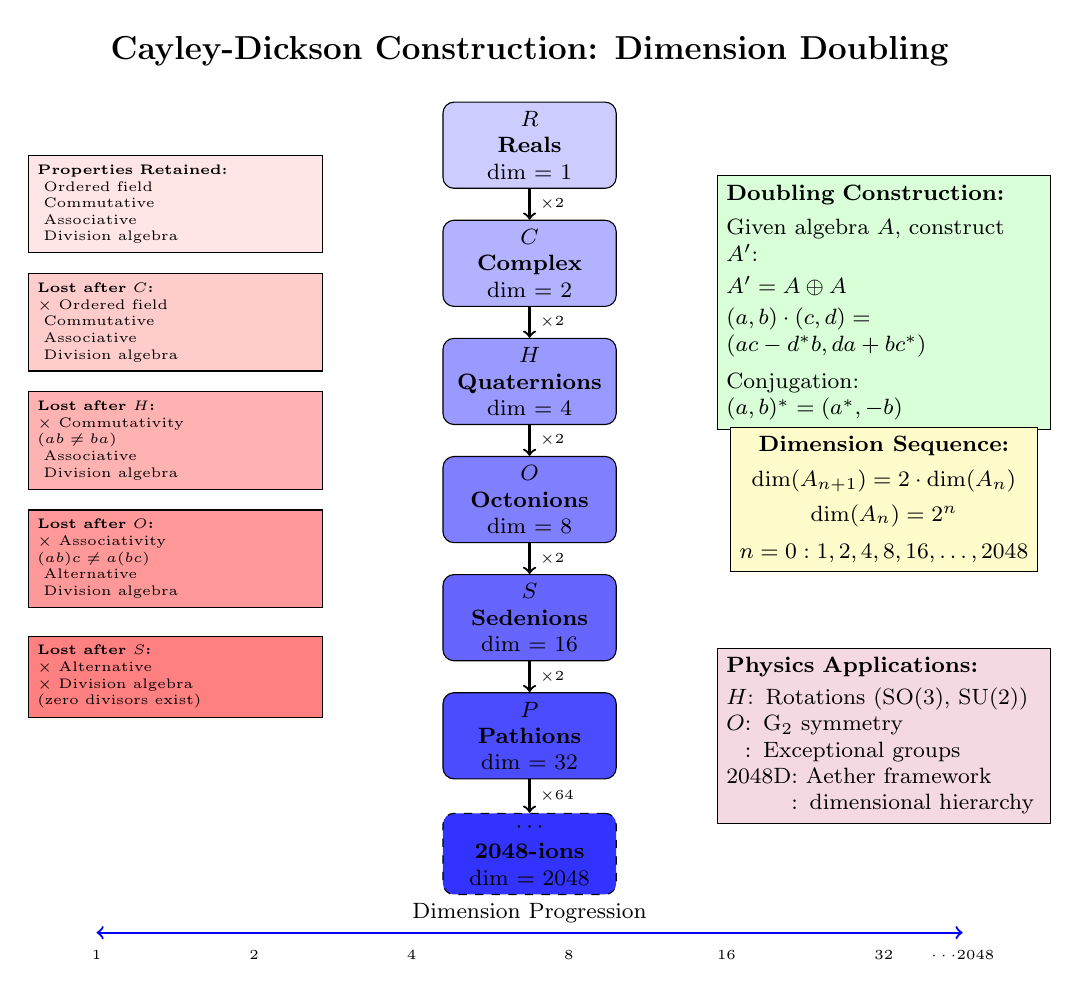
\begin{tikzpicture}[scale=1.0,
  algebra/.style={draw, rectangle, rounded corners, minimum width=2.2cm, minimum height=1cm, font=\footnotesize, align=center},
  property/.style={font=\tiny, text=red},
  arrow/.style={->, thick}]

  % Title
  \node[anchor=north, font=\large\bfseries] at (6,9.5) {Cayley-Dickson Construction: Dimension Doubling};

  % Level 0: Reals
  \node[algebra, fill=blue!20] (R) at (6,8) {
    $\mathbb{R}$ \\
    \textbf{Reals} \\
    dim = 1
  };

  % Level 1: Complex
  \node[algebra, fill=blue!30] (C) at (6,6.5) {
    $\mathbb{C}$ \\
    \textbf{Complex} \\
    dim = 2
  };

  % Level 2: Quaternions
  \node[algebra, fill=blue!40] (H) at (6,5) {
    $\mathbb{H}$ \\
    \textbf{Quaternions} \\
    dim = 4
  };

  % Level 3: Octonions
  \node[algebra, fill=blue!50] (O) at (6,3.5) {
    $\mathbb{O}$ \\
    \textbf{Octonions} \\
    dim = 8
  };

  % Level 4: Sedenions
  \node[algebra, fill=blue!60] (S) at (6,2) {
    $\mathbb{S}$ \\
    \textbf{Sedenions} \\
    dim = 16
  };

  % Level 5: Pathions
  \node[algebra, fill=blue!70] (P) at (6,0.5) {
    $\mathbb{P}$ \\
    \textbf{Pathions} \\
    dim = 32
  };

  % Level 6: Continuation
  \node[algebra, fill=blue!80, dashed] (dots) at (6,-1) {
    $\cdots$ \\
    \textbf{2048-ions} \\
    dim = 2048
  };

  % Arrows with doubling annotation
  \draw[arrow] (R) -- (C) node[midway, right, font=\tiny] {$\times 2$};
  \draw[arrow] (C) -- (H) node[midway, right, font=\tiny] {$\times 2$};
  \draw[arrow] (H) -- (O) node[midway, right, font=\tiny] {$\times 2$};
  \draw[arrow] (O) -- (S) node[midway, right, font=\tiny] {$\times 2$};
  \draw[arrow] (S) -- (P) node[midway, right, font=\tiny] {$\times 2$};
  \draw[arrow] (P) -- (dots) node[midway, right, font=\tiny] {$\times 64$};

  % Property loss cascade (LEFT SIDE)
  \node[draw, rectangle, fill=red!10, font=\tiny, align=left, text width=3.5cm] at (1.5,7.25) {
    \textbf{Properties Retained:} \\
    $\checkmark$ Ordered field \\
    $\checkmark$ Commutative \\
    $\checkmark$ Associative \\
    $\checkmark$ Division algebra
  };

  \node[draw, rectangle, fill=red!20, font=\tiny, align=left, text width=3.5cm] at (1.5,5.75) {
    \textbf{Lost after $\mathbb{C}$:} \\
    $\times$ Ordered field \\
    $\checkmark$ Commutative \\
    $\checkmark$ Associative \\
    $\checkmark$ Division algebra
  };

  \node[draw, rectangle, fill=red!30, font=\tiny, align=left, text width=3.5cm] at (1.5,4.25) {
    \textbf{Lost after $\mathbb{H}$:} \\
    $\times$ Commutativity \\
    $(ab \neq ba)$ \\
    $\checkmark$ Associative \\
    $\checkmark$ Division algebra
  };

  \node[draw, rectangle, fill=red!40, font=\tiny, align=left, text width=3.5cm] at (1.5,2.75) {
    \textbf{Lost after $\mathbb{O}$:} \\
    $\times$ Associativity \\
    $(ab)c \neq a(bc)$ \\
    $\checkmark$ Alternative \\
    $\checkmark$ Division algebra
  };

  \node[draw, rectangle, fill=red!50, font=\tiny, align=left, text width=3.5cm] at (1.5,1.25) {
    \textbf{Lost after $\mathbb{S}$:} \\
    $\times$ Alternative \\
    $\times$ Division algebra \\
    (zero divisors exist)
  };

  % Construction formula (RIGHT SIDE)
  \node[draw, rectangle, fill=green!15, font=\footnotesize, align=left, text width=4cm] at (10.5,6) {
    \textbf{Doubling Construction:} \\[3pt]
    Given algebra $A$, construct $A'$: \\[2pt]
    $A' = A \oplus A$ \\[2pt]
    $(a,b) \cdot (c,d) = $ \\
    $(ac - d^* b, da + bc^*)$ \\[4pt]
    Conjugation: \\
    $(a,b)^* = (a^*, -b)$
  };

  % Dimension formula
  \node[draw, rectangle, fill=yellow!20, font=\footnotesize, align=center] at (10.5,3.5) {
    \textbf{Dimension Sequence:} \\[3pt]
    $\dim(A_{n+1}) = 2 \cdot \dim(A_n)$ \\[3pt]
    $\dim(A_n) = 2^n$ \\[4pt]
    $n=0: 1, 2, 4, 8, 16, \ldots, 2048$
  };

  % Physics applications box
  \node[draw, rectangle, fill=purple!15, font=\footnotesize, align=left, text width=4cm] at (10.5,0.5) {
    \textbf{Physics Applications:} \\[2pt]
    $\mathbb{H}$: Rotations (SO(3), SU(2)) \\
    $\mathbb{O}$: G$_2$ symmetry \\
    \phantom{$\mathbb{O}$}: Exceptional groups \\
    2048D: Aether framework \\
    \phantom{2048D}: dimensional hierarchy
  };

  % Visual dimension progression
  \draw[thick, blue, <->] (0.5,-2) -- (11.5,-2);
  \node[below, font=\tiny] at (0.5,-2.1) {1};
  \node[below, font=\tiny] at (2.5,-2.1) {2};
  \node[below, font=\tiny] at (4.5,-2.1) {4};
  \node[below, font=\tiny] at (6.5,-2.1) {8};
  \node[below, font=\tiny] at (8.5,-2.1) {16};
  \node[below, font=\tiny] at (10.5,-2.1) {32};
  \node[below, font=\tiny] at (11.5,-2.1) {$\cdots$2048};
  \node[above, font=\footnotesize] at (6,-2) {Dimension Progression};

\end{tikzpicture}

% Usage: \input{modules/figures/fig_cayley_dickson_doubling_sequence.tex}
% Notes: Shows the full Cayley-Dickson construction from R to 2048D algebras
%        with systematic loss of algebraic properties at each doubling.
%==============================================================================

% Notes: Shows the full Cayley-Dickson construction from R to 2048D algebras
%        with systematic loss of algebraic properties at each doubling.
%==============================================================================

% Notes: Shows the full Cayley-Dickson construction from R to 2048D algebras
%        with systematic loss of algebraic properties at each doubling.
%==============================================================================

% Notes: Shows the full Cayley-Dickson construction from R to 2048D algebras
%        with systematic loss of algebraic properties at each doubling.
%==============================================================================
